\begin{frame}
recap
    class / object - fundamental unit of state natural to parallel algo\\
    method - fundamental unit of execution in parallel algo\\
unit of functionality = class
unit of state = obj
unit of execution = function / method
\end{frame}


\begin{frame}
  \frametitle{Messages ...
    \only<1>{help objects communicate}
    \only<2>{express algorithmic dependencies}
    \only<3>{drive the parallel computation}
  }
  \begin{figure}
  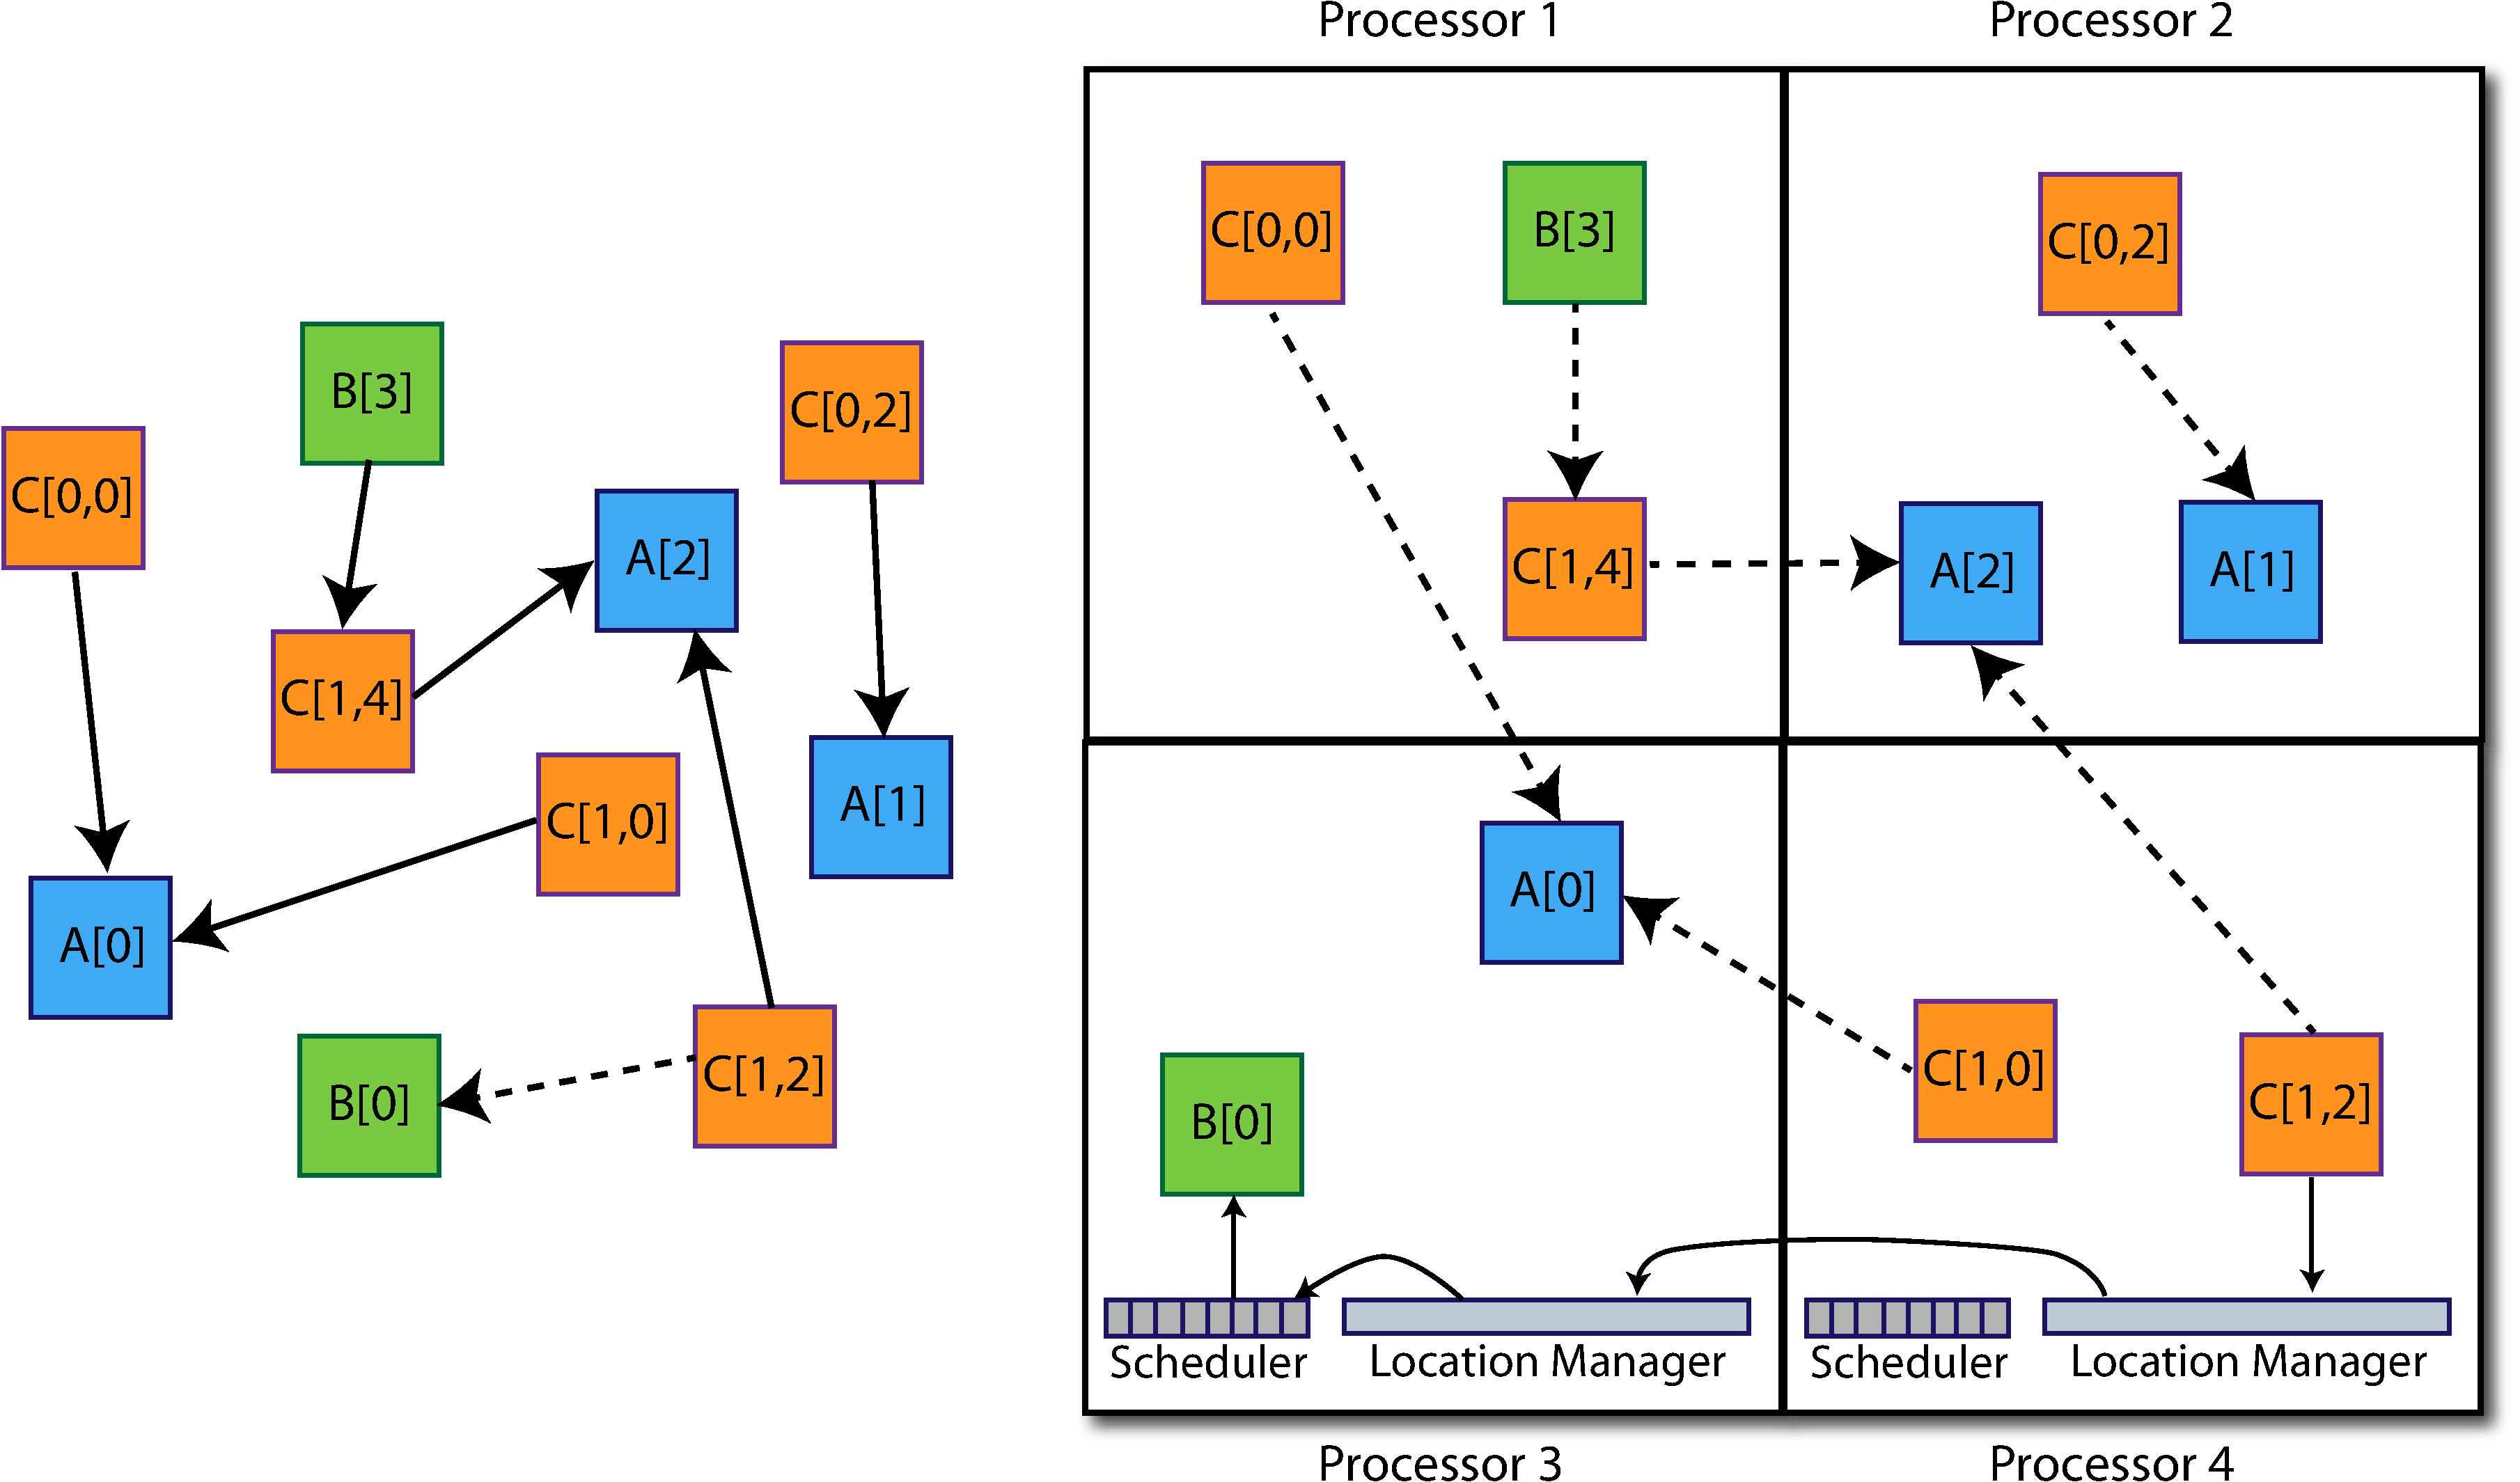
\includegraphics[trim=0in 0in 14in 2in, clip=true, height=0.85\textheight]{../figures/elements2.pdf}
  \end{figure}
\end{frame}


\begin{frame}
  \frametitle{Messages ...
    \only<1>{wait in queues}
    \only<2>{and are scheduled for execution}
  }
  \begin{center}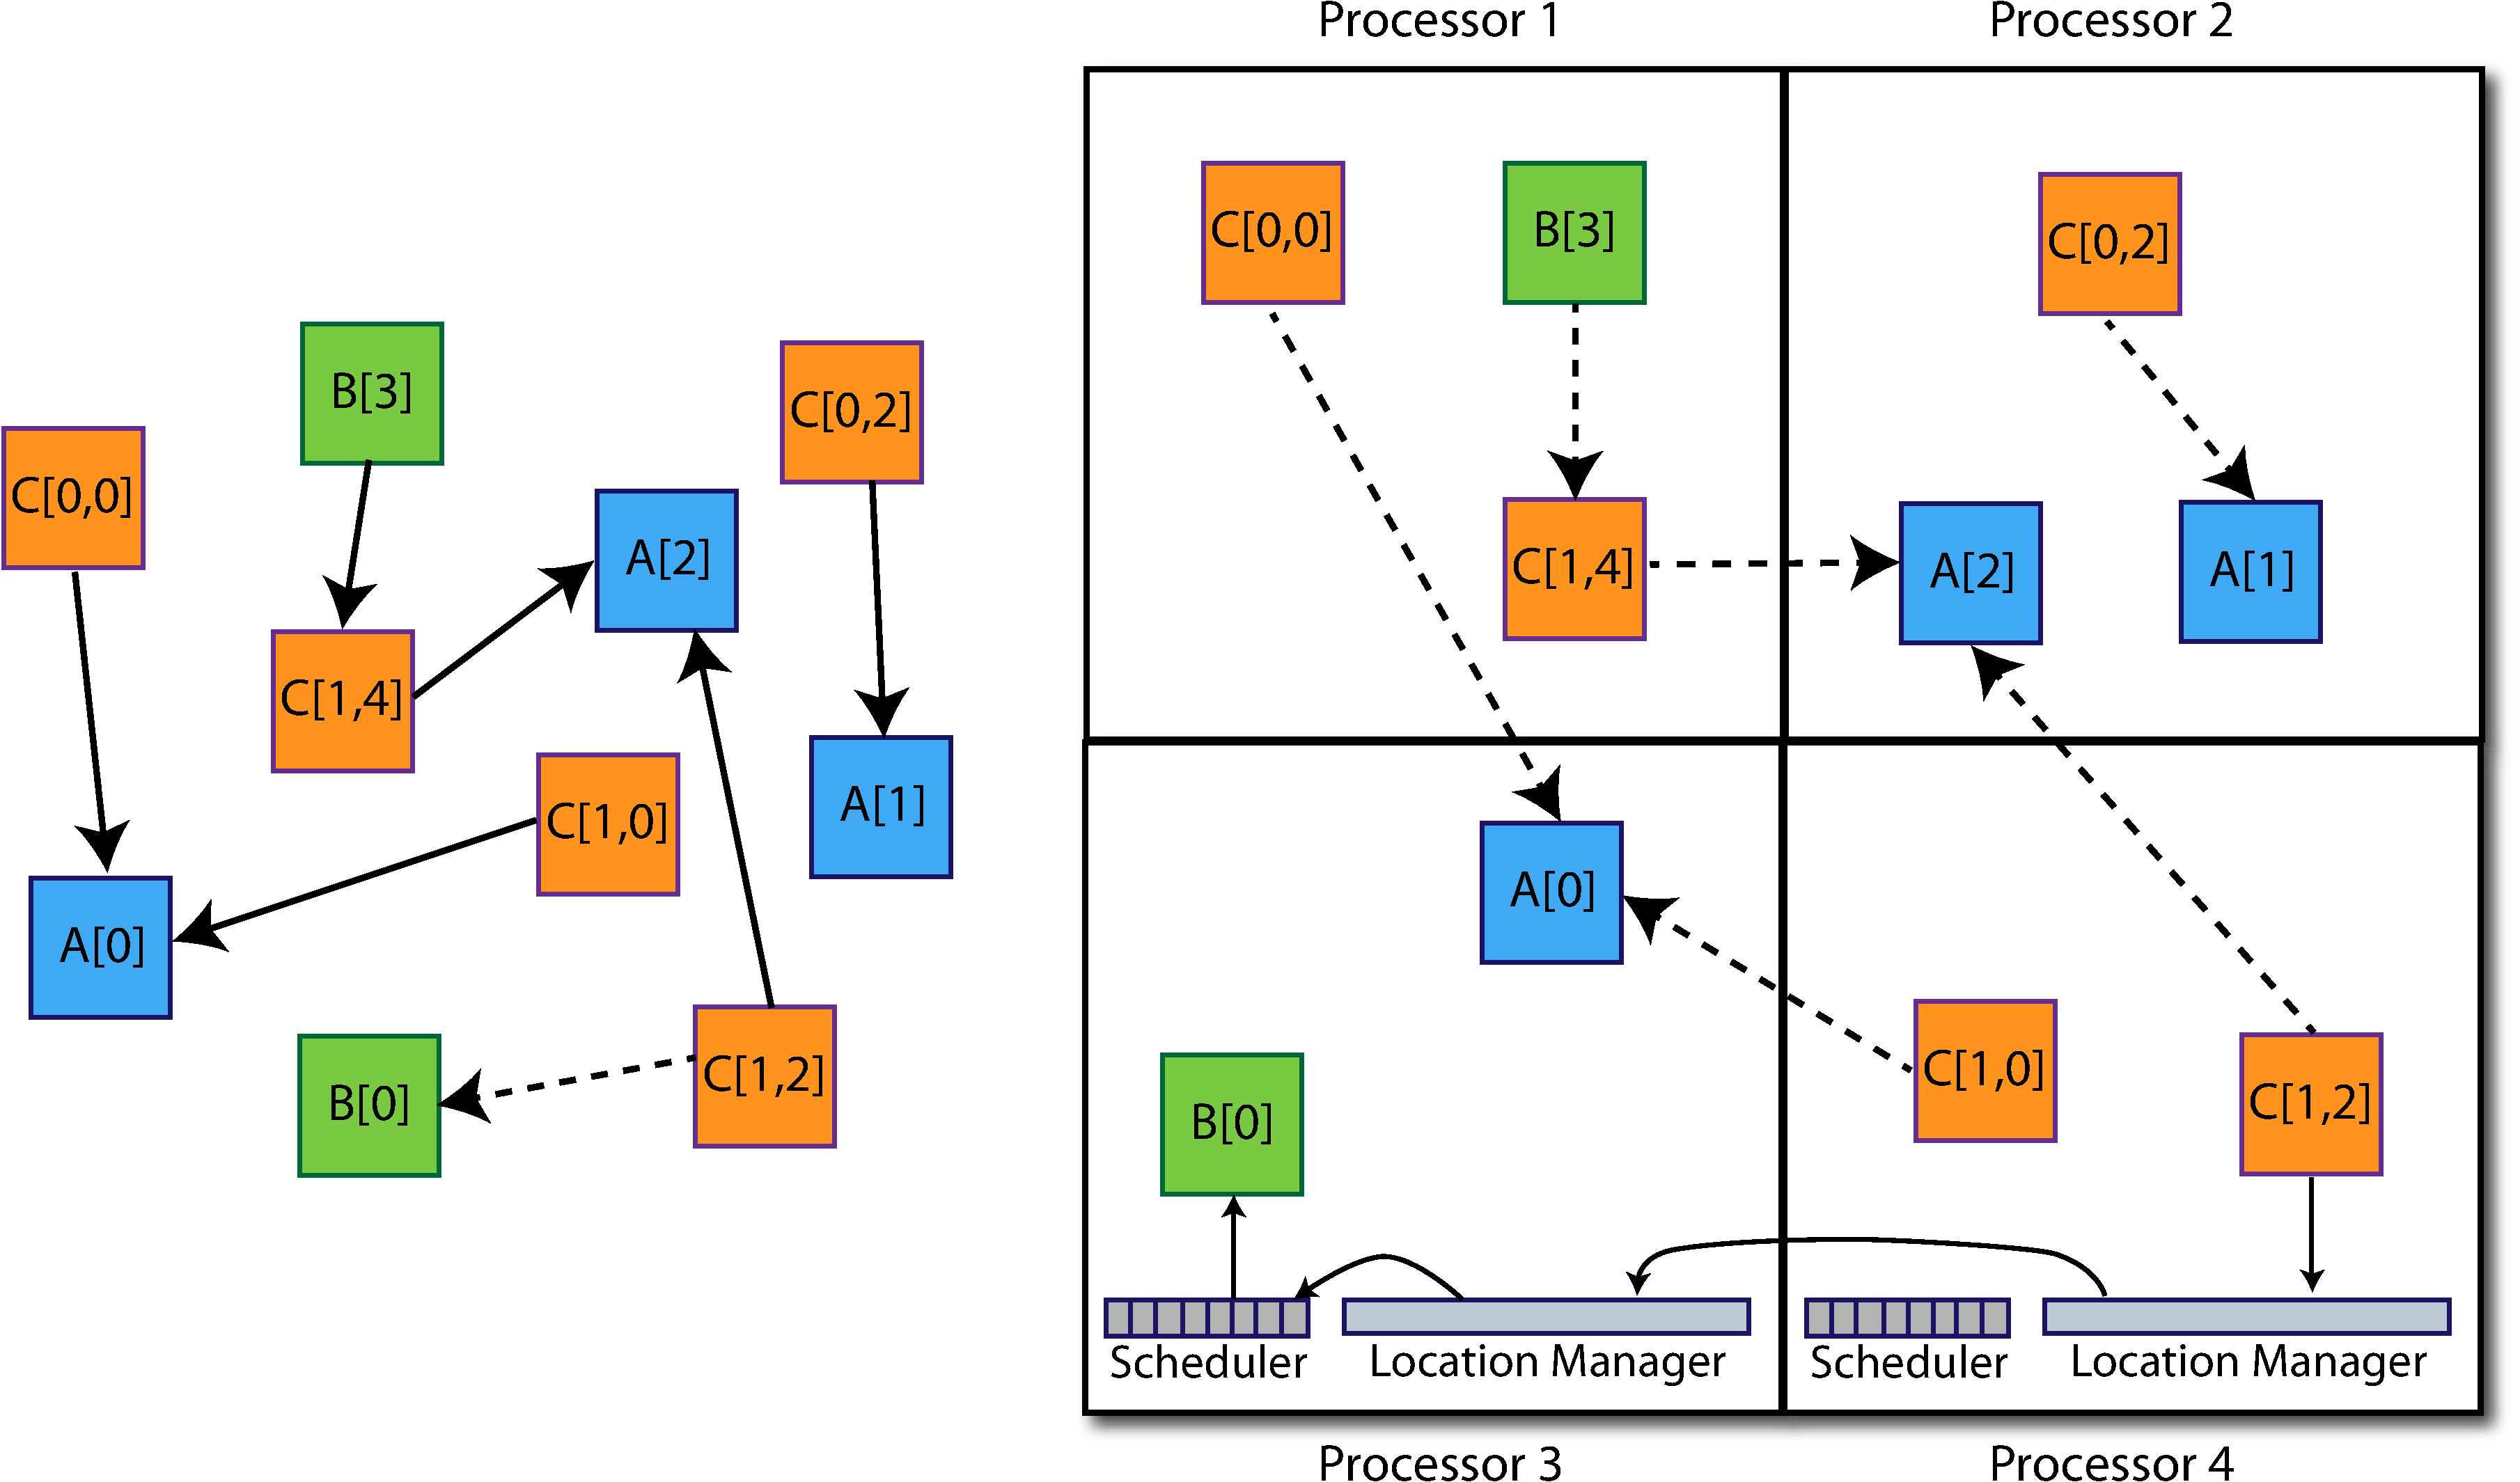
\includegraphics[width=0.9\textwidth]{../figures/elements2.pdf}\end{center}
\end{frame}



